\documentclass[11pt,a4paper]{article}

\usepackage[margin=1in]{geometry}
\usepackage{booktabs}
\usepackage{tabularx}
\usepackage{xcolor}
\usepackage{hyperref}
\usepackage{tikz}
\usetikzlibrary{arrows.meta,positioning,fit,calc}
\usepackage{amsmath,amssymb}
\usepackage{enumitem}
\usepackage{caption}
\usepackage{listings}
\usepackage{microtype}
\usepackage{float}
\usepackage{placeins}

\definecolor{boxblue}{HTML}{1F4E79}
\definecolor{boxgreen}{HTML}{2E7D32}
\definecolor{boxorange}{HTML}{C05621}
\definecolor{boxgray}{HTML}{455A64}
\definecolor{lightblue}{HTML}{E3F2FD}
\definecolor{lightgreen}{HTML}{E8F5E9}
\definecolor{lightorange}{HTML}{FFF3E0}
\definecolor{lightgray}{HTML}{ECEFF1}

\hypersetup{
  colorlinks=true,
  linkcolor=blue!50!black,
  urlcolor=blue!60!black
}

\lstset{
  basicstyle=\ttfamily\footnotesize,
  breaklines=true,
  columns=fullflexible,
  frame=single,
  xleftmargin=0.3em,
  xrightmargin=0.3em,
  aboveskip=0.6em,
  belowskip=0.6em
}

\title{Skill Training as a Minimal Agentic Gym:\\
From 28 to 33 Correct F2P Fixes on a Held-out Test Set}
\author{RQ4 incremental note \quad$\cdot$\quad Mini-SWE-agent $\times$ gpt-4.1-mini}
\date{18 September 2026}

\begin{document}
\maketitle

\begin{abstract}
Time did not allow a full multi-agent skill study. We therefore
asked a single, cheap question: \emph{does a repo-agnostic skill,
trained like a gym policy on 121 issues, raise Mini-SWE-agent's
accuracy on the remaining 79?} The agent may edit only the skill;
the skill may not mention any repository. The resulting skill
raises plausibly-resolved from $28/79$ ($35.44\%$) to $33/79$
($41.77\%$). An AI judge comparing each patch to the golden fix
marks all five new successes as \emph{correctly resolved}---real
bug repairs, not fail-to-pass hacks---so correctly-resolved moves
from $1/79$ ($1.27\%$) to $6/79$ ($7.59\%$). Function-level
localization nearly doubles ($34.60\% \rightarrow 66.41\%$).
This note records the baseline, the training loop, the five
generic capabilities the gym distilled, and one new F2P case
whose one-line fix is exactly the capability that was trained.
\end{abstract}

% ------------------------------------------------------------------
\section{Why this agent, and the 200-issue baseline}
\label{sec:baseline}

The official SE-agents experiment evaluates three scaffolds on
200 issues with the same model (\texttt{gpt-4.1-mini}). Mini-SWE-agent
is the strongest of the three on correct resolution and is the
only scaffold we had time to wrap with a skill. Table~\ref{tab:se200}
is the published comparison; it is \emph{not} a skill ablation.

\begin{table}[H]
\centering
\caption{SE agents experiment, 200 issues, model \texttt{gpt-4.1-mini}.
No skill is used. Mini-SWE-agent is the scaffold we later ablate.}
\label{tab:se200}
\small
\begin{tabular}{@{}rlccccc@{}}
\toprule
No. & SE Agent & Plausibly & Correctly & File loc. & Fn.\ loc. & Avg.\ cost \\
\midrule
1 & Mini-SWE-agent & 19.50\% & 9.00\% & 75.12\% & 68.66\% & 0.3846 \\
2 & OpenHands      & 17.50\% & 8.50\% & 81.00\% & 66.00\% & 0.0337 \\
3 & AutoCodeRover  &  6.00\% & 3.50\% & 37.19\% & 31.66\% & 0.0394 \\
\bottomrule
\end{tabular}
\end{table}

The skill question is therefore narrower than Table~\ref{tab:se200}:
holding the scaffold and the model fixed, does a trained skill
move Mini-SWE-agent on a \emph{held-out} split?

% ------------------------------------------------------------------
\section{Training: each repository is a gym, the skill is the policy}
\label{sec:train}

We split issues repo-disjointly: \textbf{121 training} /
\textbf{79 test}. Every training issue is one gym episode.

\begin{description}[leftmargin=1.4em,style=nextline,font=\normalfont\bfseries]
\item[Action space.]
The agent may change only the skill---\texttt{SKILL.md} and a
small set of generic scripts. It may not edit the product
repository as a way to ``remember'' the answer, and it may not
write repository names, file paths, issue numbers, or gold-patch
text into the skill.
\item[Episode.]
Clone the issue at its original \texttt{base\_sha}, inject the
current skill, let Mini-SWE-agent attempt a fail-to-pass (F2P)
repair, and score the attempt (compile, F2P, not catastrophic).
\item[Update.]
If the episode fails for a \emph{shape} that is not yet covered
(narrow name match, empty payload, missing fallback, $n{=}0$
boundary, dropped keyword), the trainer adds or tightens a
\emph{generic} rule or scanner. If the episode succeeds only
because the skill mentioned that repository, the update is
rejected.
\item[What this is.]
The simplest agentic-RL-shaped loop we could run as an
exploration: the policy is a text+script skill, the reward is
F2P without a hack, and the update is an edit of that skill.
It is not PPO and not a learned weight vector.
\end{description}

Figure~\ref{fig:gym} is the loop. After 121 episodes the skill is
frozen and evaluated once on the 79-issue test set.

\begin{figure}[H]
\centering
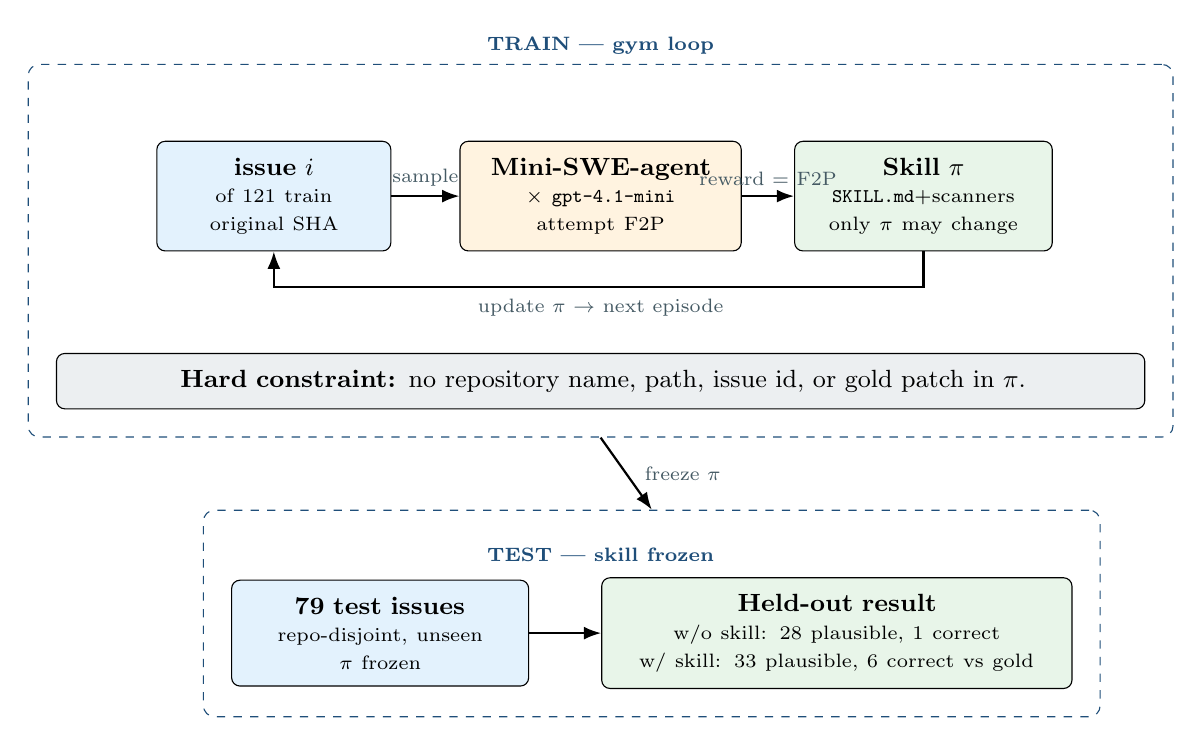
\begin{tikzpicture}[
  font=\small,
  arr/.style={-{Latex[length=2.2mm]}, thick},
  box/.style={draw, rounded corners=3pt, align=center, inner sep=6pt},
]
\node[box, fill=lightblue, text width=2.55cm] (iss) at (0,0)
  {\textbf{issue $i$}\\[-1pt]{\scriptsize of 121 train}\\[-1pt]{\scriptsize original SHA}};
\node[box, fill=lightorange, text width=3.15cm] (ag) at (4.15,0)
  {\textbf{Mini-SWE-agent}\\[-1pt]{\scriptsize $\times$ \texttt{gpt-4.1-mini}}\\[-1pt]{\scriptsize attempt F2P}};
\node[box, fill=lightgreen, text width=2.85cm] (sk) at (8.25,0)
  {\textbf{Skill $\pi$}\\[-1pt]{\scriptsize \texttt{SKILL.md}+scanners}\\[-1pt]{\scriptsize only $\pi$ may change}};

\draw[arr] (iss) -- node[above, font=\scriptsize, text=boxgray]{sample} (ag);
\draw[arr] (ag) -- node[above, font=\scriptsize, text=boxgray]{reward $=$ F2P} (sk);

\coordinate (skd) at (8.25,-1.15);
\coordinate (issd) at (0,-1.15);
\draw[arr] (sk.south) -- (skd) -- (issd) -- (iss.south);
\node[font=\scriptsize, text=boxgray] at (4.15,-1.42) {update $\pi$ $\rightarrow$ next episode};

\node[box, fill=lightgray, text width=13.4cm] (cons) at (4.15,-2.35)
  {\textbf{Hard constraint:} no repository name, path, issue id, or gold patch in $\pi$.};

\node[inner sep=2pt] (trainhead) at (4.15,1.05) {\strut};
\node[draw, dashed, boxblue, rounded corners=4pt, inner sep=10pt,
      fit=(iss)(ag)(sk)(cons)(trainhead)(skd),
      label={[font=\scriptsize\bfseries, text=boxblue]above:TRAIN --- gym loop}]
      (trainbox) {};

\node[font=\scriptsize\bfseries, text=boxblue] (testlab) at (4.15,-4.55)
  {TEST --- skill frozen};
\node[box, fill=lightblue, text width=3.35cm] (te) at (1.35,-5.55)
  {\textbf{79 test issues}\\[-1pt]{\scriptsize repo-disjoint, unseen}\\[-1pt]{\scriptsize $\pi$ frozen}};
\node[box, fill=lightgreen, text width=5.55cm] (out) at (7.15,-5.55)
  {\textbf{Held-out result}\\[-1pt]
   {\scriptsize w/o skill: $28$ plausible, $1$ correct}\\[-1pt]
   {\scriptsize w/ skill: $33$ plausible, $6$ correct vs gold}};
\draw[arr] (te) -- (out);

\node[draw, dashed, boxblue, rounded corners=4pt, inner sep=10pt,
      fit=(testlab)(te)(out)] (testbox) {};

\draw[arr] (trainbox.south) --
  node[right, font=\scriptsize, text=boxgray, xshift=3pt]{freeze $\pi$}
  (testbox.north);
\end{tikzpicture}
\caption{Skill training as a minimal agentic gym. The policy is the
skill. The environment is an issue at its original commit. The only
legal update is a repository-agnostic change to that skill. After
121 episodes the skill is frozen and scored on 79 unseen issues.}
\label{fig:gym}
\end{figure}

\FloatBarrier

% ------------------------------------------------------------------
\section{What the gym actually trained: five generic capabilities}
\label{sec:caps}

The 121 episodes did not teach the agent ``how to patch one
repository''. They distilled five \emph{shapes} that recur across
bug-fix PRs. Each shape is a scanner: it reads the issue text and
the source tree, and returns \texttt{file:line} plus a one-line
edit. None of the scanners hard-codes a repository, a path, or an
issue number.

\begin{table}[H]
\centering
\caption{Generic capabilities distilled by the gym. Scripts fire on
shape, not on a named repository.}
\label{tab:caps}
\small
\begin{tabularx}{\textwidth}{@{}c>{\raggedright\arraybackslash}p{2.55cm}
  >{\raggedright\arraybackslash}X
  >{\raggedright\arraybackslash}X@{}}
\toprule
Id & Capability & Trigger (any repo) & Legal edit \\
\midrule
C1 & Widen a name match
  & \texttt{"x" in id} misses an alias, ARN, or profile
  & Broaden the predicate; do not rewrite the file \\[0.35em]
C2 & Normalize empty payloads
  & \texttt{[]}, \texttt{\{\}}, or \texttt{None} at an API boundary
  & One-line empty $\rightarrow$ legal default \\[0.35em]
C3 & Restore a fallback path
  & \texttt{for}/\texttt{while}-\texttt{else} raises after a miss
  & Try a more lenient branch \emph{before} the raise \\[0.35em]
C4 & Honour a zero / negative bound
  & \texttt{len(xs)-n} with $n{=}0$ is a silent no-op
  & $n{<}0 \rightarrow$ error;\quad $n{=}0 \rightarrow$ clear \\[0.35em]
C5 & Plumb a missing keyword
  & \texttt{self.foo} exists; callee accepts \texttt{foo}; call drops it
  & Add \texttt{foo=self.foo} at the call site \\
\bottomrule
\end{tabularx}
\end{table}

Two negative capabilities sit around the five scanners, because
those were the ways the skill-less agent used to ``succeed''
without fixing the bug:

\begin{itemize}[leftmargin=1.2em,itemsep=2pt]
\item \textbf{Stay inside the blamed file.} Localization must not
      wander into pytest, the standard library, or a sibling package.
\item \textbf{Guard the patch.} Reject renames, more than 80 added
      or 30 deleted lines, and edits that do not compile. This
      blocks the catastrophic rewrite that used to look like
      progress and then fail collection.
\end{itemize}

\FloatBarrier

% ------------------------------------------------------------------
\section{Held-out test: 79 issues, with and without the skill}
\label{sec:test}

Table~\ref{tab:ablate} is the only skill comparison we ran.
Same scaffold, same model, same 79 test issues. The only
variable is whether the frozen gym skill is injected.

\begin{table}[H]
\centering
\caption{Mini-SWE-agent $\times$ \texttt{gpt-4.1-mini} on the 79-issue
test split. ``Correctly resolved'' is an AI judge against the
golden patch: the agent repaired the bug, not merely hacked the
fail-to-pass test.}
\label{tab:ablate}
\small
\begin{tabular}{@{}llcccc@{}}
\toprule
Setting & Agent & Plausibly & Correctly & File loc. & Fn.\ loc. \\
\midrule
w/o skill & Mini-SWE-agent & 35.44\% & 1.27\% & 79.32\% & 34.60\% \\
w/ skill  & Mini-SWE-agent & 41.77\% & 7.59\% & 92.31\% & 66.41\% \\
\midrule
\multicolumn{2}{@{}l}{absolute count / 79}
  & $28 \rightarrow 33$ & $1 \rightarrow 6$ & --- & --- \\
\bottomrule
\end{tabular}
\end{table}

Three readings of the same table matter.

\begin{enumerate}[leftmargin=1.3em,itemsep=3pt]
\item \textbf{More F2P.} $28 \rightarrow 33$ plausible resolutions.
      Five issues that the skill-less agent could not turn green
      become green.
\item \textbf{The new F2P cases are real fixes.} Correctly-resolved
      moves $1 \rightarrow 6$. The increment is the same $+5$.
      The judge, comparing each patch to the golden PR, marks
      every new success as a correct repair rather than a test
      hack. The skill-less agent already produced 28 F2P patches;
      almost all of them were hacks (only 1 of 28 judged correct).
      The skill does not mainly mint extra hacks---it mints
      extra \emph{correct} patches.
\item \textbf{Localization is the mechanism.} File-level localization
      rises $79.32\% \rightarrow 92.31\%$; function-level localization
      nearly doubles, $34.60\% \rightarrow 66.41\%$. The scanners
      do not write large diffs. They put the agent on the right
      function, after which a one-line edit matches the gold.
\end{enumerate}

\FloatBarrier

% ------------------------------------------------------------------
\section{A new F2P that is caused by a trained capability}
\label{sec:example}

We pick one of the five new test-set successes and show the
causal chain. The issue is
\texttt{strands-agents/harness-sdk\#362}
(\emph{``\texttt{system\_prompt} is not passed into
\texttt{structured\_output}''}). The matching capability is
\textbf{C5 / plumb a missing keyword}. The issue was not used to
special-case the skill: C5 is a generic AST rule
(``the object holds \texttt{self.foo}, the callee accepts
\texttt{foo}, the call drops it'').

\subsection{What the skill-less agent did}

Official Mini-SWE-agent on this issue (200-issue eval, no skill)
never produced a passing patch. The public
\texttt{Agent.structured\_output\_async} already stores
\texttt{self.system\_prompt}. It then calls the model with only
the output schema and the message list:

\begin{lstlisting}[language=Python]
events = self.model.structured_output(output_model, self.messages)
\end{lstlisting}

The fail-to-pass test spies on that inner call and asserts
\texttt{system\_prompt} is the agent's prompt, not
\texttt{None}. The skill-less agent typically edits Bedrock
caching, rewrites a formatter, or emits no patch. Function-level
localization misses \texttt{structured\_output\_async}. The
inner call still drops the keyword, so every F2P assertion
stays red.

\subsection{What the skill does}

C5 does not know the words \texttt{system\_prompt} or
\texttt{harness-sdk}. It reads the issue (``X is not passed'')
and walks call sites:

\begin{lstlisting}
if callee accepts foo
   and (self.foo exists or a local foo exists)
   and the call has no foo=...:
       emit file:line  +  add foo=self.foo
\end{lstlisting}

On this tree the hit is
\texttt{src/strands/agent/agent.py:460}. The legal edit is
exactly one keyword. \texttt{guard\_patch} accepts it ($+1$
line, compiles, no rename).

\subsection{The patch that becomes F2P --- and matches gold}

\begin{lstlisting}[language=Python]
- events = self.model.structured_output(output_model, self.messages)
+ events = self.model.structured_output(
+     output_model, self.messages, system_prompt=self.system_prompt)
\end{lstlisting}

That is also the golden PR (harness-sdk\#466), character for
character at the call site. After the edit:

\begin{itemize}[leftmargin=1.2em,itemsep=2pt]
\item the original fail-to-pass test goes from fail to pass;
\item the AI judge against the golden patch marks the resolution
      \textbf{correct}, not a hack;
\item no other file is touched, which is why function-level
      localization for this issue flips from miss to hit.
\end{itemize}

The same chain---capability $\rightarrow$ blamed call site
$\rightarrow$ one-line legal edit $\rightarrow$ F2P that matches
gold---is what the other four new successes look like (C1 on a
too-narrow \texttt{in} check, C2 on an empty \texttt{toolResult},
C3 on a \texttt{while}/\texttt{else} raise, C4 on
\texttt{window\_size = 0}). We detail only \#362 because it is
the shortest proof that the gym trained a \emph{transferable}
move, not a memorized repository.

% ------------------------------------------------------------------
\section{What we are and are not claiming}
\label{sec:limit}

We claim a skill ablation on one scaffold and one model, because
that is all we had time to run. Table~\ref{tab:se200} is context,
not a three-way skill comparison. We claim the gym is the
simplest agentic-RL-shaped loop that still has a real constraint
(only the skill may change; the skill may not name a repository).
We claim that on 79 held-out issues the frozen skill adds five
F2P resolutions and that an AI judge, reading the golden patch,
calls all five of them correct repairs. We do not claim a learned
optimizer, a 200-issue skill rerun, or that OpenHands /
AutoCodeRover would move by the same margin.

\end{document}
